\section{Evaluation}\label{sec:evaluation}

\subsection{Domains Setup}

%\subsubsection{Domains}

\begin{table}
	\caption{Continuum Setup for the Experimental Evaluation}
	\label{tab:domain-exp-config}
	\begin{tabular*}{1\textwidth}{@{\extracolsep{\fill}}>{\raggedright}p{1.5cm}>{\raggedright}p{6cm}>{\raggedright}p{6cm}}
		\toprule 
		Domain & Machine Resources & Execution Environment\tabularnewline
		\midrule
		\midrule 
		Edge-Local & ubuntu/trusty64-2, 4x vCPUs, 4Gb RAM & Openwhisk, 256 Mb/Action, Python 2.7 + OpenCV \tabularnewline
		\midrule 
		Edge-Mobile & ubuntu/trusty64-2, 8x vCPUs, 16Gb RAM & Openwhisk, 256 Mb/Action, Python 2.7 + OpenCV \tabularnewline
		\midrule 
		Cloud-FaaS & N/A & AWS Lambda, 256 Mb/Function, Python 2.7 + OpenCV \tabularnewline
		\midrule 
		Cloud-IaaS & Autos Scaling Group with t2.micro instances + Amazon Linux AMI 2017  & NodeJs 6.11 server + Python 2.7 + OpenCv \tabularnewline
		\bottomrule
	\end{tabular*}
\end{table}

Table~\ref{tab:domain-exp-config} shows the different domains that were deployed to materialize the computational continuum for the experiments. Edge domains feature the Apache Openwhisk (formerly IBM Openwhisk) serverless framework\footnote{https://openwhisk.incubator.apache.org/} that manages {\em actions} (equivalent to functions). Being open-source, openwhisk is (to date) the only serverless alternative among the major vendors that can be deployed locally or on private clouds. 
%Particularly, openwhisk provides a built-in noSQL database: CouchDB, which is associated with the implemented actions through user-defined triggers and rules. 
Particularly, Edge-local domain is always placed close to the client applications/devices (one or two network hops). This deployment allows us to represent a situation where latency is close to zero, but the computational resources are highly constrained, as scaling-up is not possible due to inherent physical restrictions of the underlying infrastructure. Similarly, the Edge-mobile domain is placed on an university server, where the computational resources are less constrained, and still low latency can be achieved due to physical proximity and data locality. Note that in both cases the domains are deployed in the same LAN that originates the requests, to emulate the few-hop scenario in which devices are directly connected to their nearest Edge domains.


%In this experiment, we considered two alternatives for deploying the serverless continuum architecture, mimicking the behavior of both an edge node and a fog node (Figure~\ref{fig:exp-edge}).  

%The client application is embedded in the edge node, consisting on the postman requests and the node.js endpoint (Figure~\ref{fig:exp-setup1}). 
%On the edge-local alternative, we used a virtual machine running locally, on a regular laptop, with 4x CPU, 4x Gb of RAM and 40 Gb SSD of storage. 

%For the Fog alternative, we deployed the serverless architecture on Policloud\footnote{http://policloud.polimi.it/}, the private IaaS solution of Politecnico di Milano. Here, the computational resources are less constrained, and still low latency can be achieved due to physical proximity (two hops from the client) and data locality. This setup runs on a small cluster of 4 virtual machines with 2x CPU, 4x Gb of Ram and 100 GB SSD, each running a different component of openwhisk (triggers and storage, Http server, controller, and invokers, respectively). Note that in this case the fog node is deployed in the same LAN that originates the requests, to emulate the few-hop scenario in which devices are directly connected to their corresponding MEC.

The serverless cloud alternative (Cloud-FaaS) for this experiment uses AWS Lambda\footnote{https://aws.amazon.com/lambda/} as the first-available and most mature serverless solution in the market. The functions and associated libraries and services (storage, image recognition) are hosted in the same region, which is enforced by AWS to guarantee a certain degree of data locality. Finally, we also deployed the feature recognition functionality as a ``serverful'' Cloud setup (Cloud-IaaS). However, the main goal of this experiment is not to compare traditional cloud services against a serverless solution, but to demonstrate that the proposed continuum can outperform the Cloud under certain circumstances and requirements.


\subsection{Latency} 

In order to compare the latency along the continuum, we performed experiments with a fixed number of requests (extraction and matching of features from a sample image) in a fixed interval, and without using the A3-E middleware, since they were aimed to evaluate only the different domains.

Figure~\ref{fig:exp-setup1} shows the experimental setup. Capturing and uploading an image is emulated using Postman\footnote{https://www.getpostman.com/}, a JavaScript open source application designed to load test functional behaviors and measure the performance of Web APIs. The  payload for this experiment was a sample image of approximately 65 Kb, which is a reasonable size for this use case considering the requirements regarding low-latency, computation time and battery consumption~\cite{rodriguez16mobile}. 

Then, the image is sent through HTTP/POST and different subsequent steps are executed depending on the domain: Openwhisk actions for both Edge domains, AWS Lambda functions for Cloud-FaaS domain, and a simple Nodejs server that calls a Python function for Cloud-IaaS domain.

%In our edge domains for the experiment, uploading an image to CouchDB (Step 3.a) triggers the action that performs the feature extraction and matching (Step 4.a)  with the points-of-interest, supported by the OpenCV\footnote{\url{http://opencv.org}} visual recognition library (Step 5.a). 


\begin{figure}
	
	\centering
	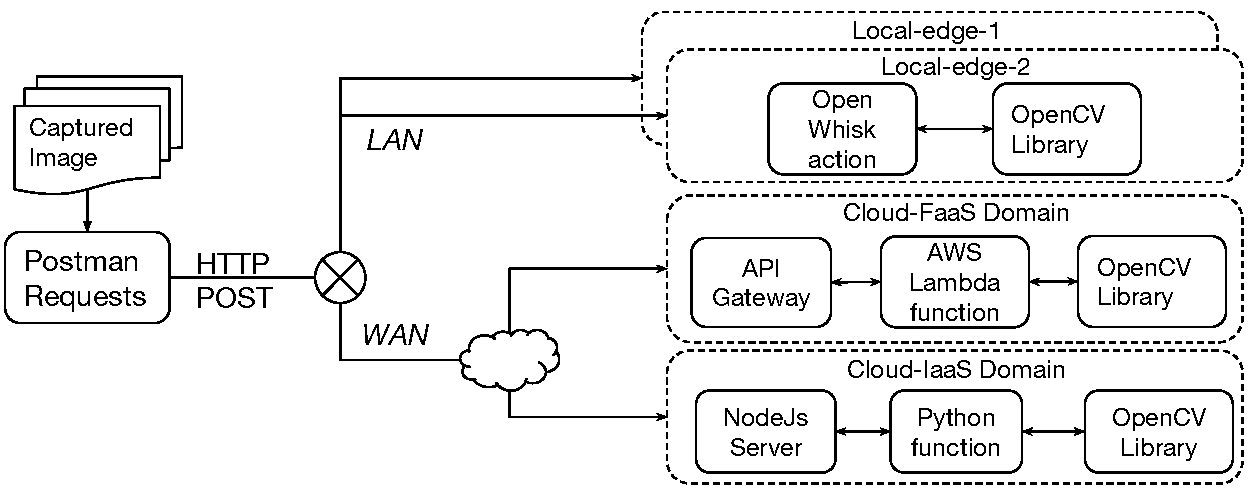
\includegraphics[width=0.9\textwidth]{figs/experimental-setup.pdf}
	\caption{Setup for Latency Experiments}
	\label{fig:exp-setup1}
\end{figure}

\subsubsection{Baseline Latency}

To measure the baseline latency, the workload was parameterized as 100 requests fired at a constant rate (two per second), considering not only the default maximum for concurrent executions in AWS Lambda\footnote{http://docs.aws.amazon.com/lambda/latest/dg/concurrent-executions.html} and Openwhisk\footnote{https://github.com/apache/incubator-openwhisk/blob/master/docs/reference.md}, but also the limited resources of the edge domains. This was done in order to avoid stressing any of the servers and measure relative latency under normal operation. Figure~\ref{fig:baseline-latency} shows the average latency and standard deviation over 5 executions of 100 calls each. These results do not consider the actual computation time (which will be discussed in the following experiments), but the overhead of network communication per call. 

\begin{figure}
	
	\centering
	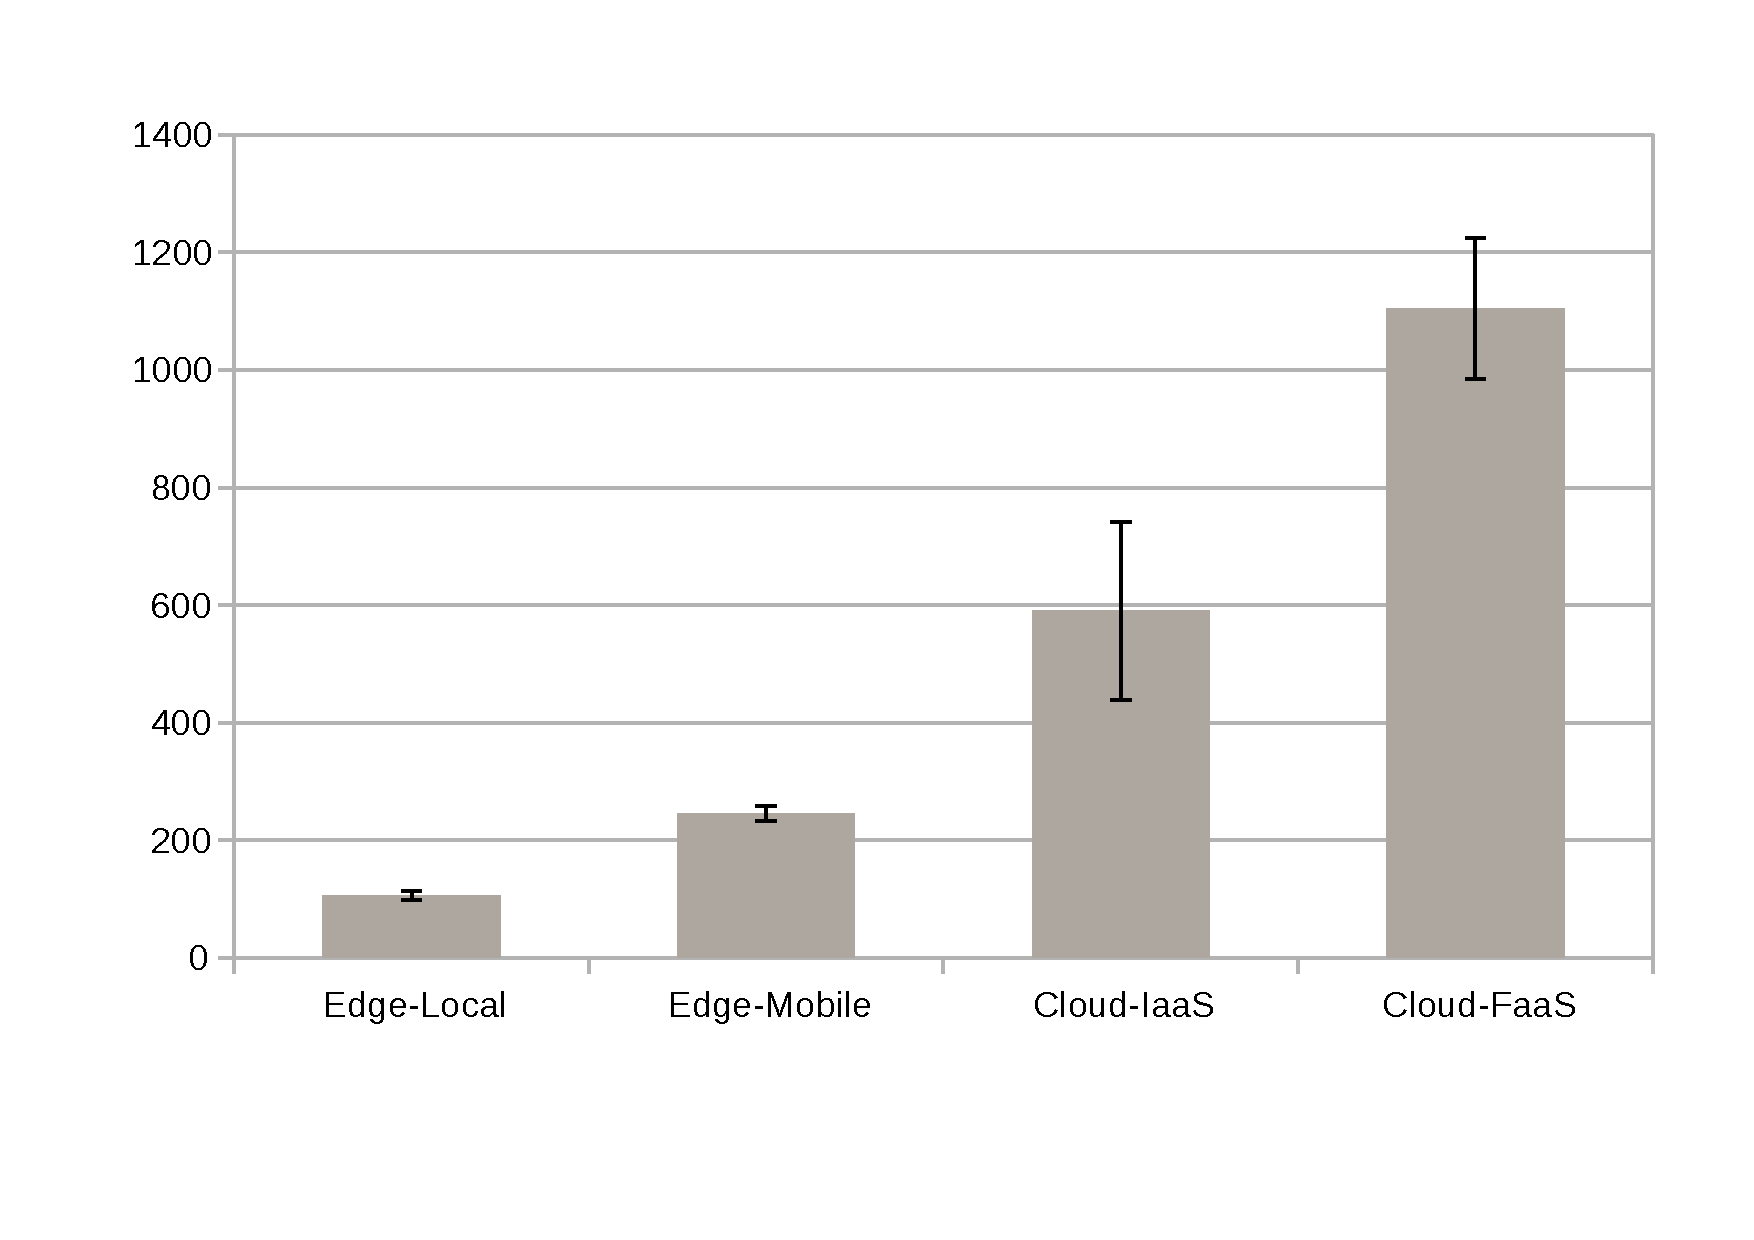
\includegraphics[width=0.6\textwidth]{figs/latency-baseline}
	\caption{Baseline latency results for different domains.}
	\label{fig:baseline-latency}
\end{figure}

 For this scenario, the latency added by the edge domains is less than the latency in both cloud alternatives. Regarding the serverless cloud alternative, the reduction in latency is 90\% for edge-local and 82\% for edge-mobile respectively, whilst for the traditional cloud domain the reduction is 77\% and 58\% respectively. 
 
 The edge-local domain outperformed all the other alternatives for this scenario, but at the same time is the most resource-constrained, which hinders its availability under heavier workloads, as it will be seen in the stress tests. Interestingly, the traditional cloud domain also outperformed the serverless one (46\% less latency); this can be due to the additional steps performed by the API Gateway in order to forward RESTful calls to lambda functions\footnote{http://docs.aws.amazon.com/lambda/latest/dg/with-on-demand-https.html}. Nevertheless, this advantage is mitigated by the fact that the serverless alternative is more reactive against bursts of workload, scaling automatically and offering a fine-grained cost model~\cite{Villamizar2017lambda,Hendrickson:2016}.

\subsubsection{Stress Tests}

%We could fire like 100 requests and measure the latency of each one and later have the average and the 
\subsubsection{Discussion}



\subsection{Battery} The second set of experiments targeted the measurement of battery consumption of a mobile device in two scenarios: 1) in which feature extraction and matching were performed locally, and 2) these tasks were offloaded to edge servers.

\subsection{Continuum} The third and final set of experiments targeted the evaluation of A3-E with a computational continuum scenario. In specific, the evaluation consisted of a mobile device hosting a simplified version of an AR application with the feature extraction and matching modeled as stateless functions that can be executed locally (Java Functions), in an edge-based FaaS platform (OpenWhisk), or a cloud-based FaaS platform (Amazon Lambda).